\chapter{Portable Executable Format} \label{chap:peformat}

The \PE{} is a file format for image files used by Microsoft products for 32- and 64-bit system architectures. It is the successor of the \NZ{} file format for 16-bit systems. The \PE{} format is described in the \PECOFF{} \cite{pespec}

\PE{} file types, which are relevant for this thesis, are \DLL{} and \EXE{} files. \DLL{} files export functions or data other programs can use. They can have various file endings, including \emph{.sys}, \emph{.dll}, \emph{ocx}, \emph{.cpl} and \emph{.drv}. (\cf{} \cite{micrdll}) A \DLL{} is loaded into the context of another process.
\EXE{} files have the file ending \emph{.exe}. They usually don't export any symbols. The system creates a new process upon launching the \EXE{}.
The system recognizes the file type by a certain flag in the \PE{} headers. (see page~\pageref{dllflag}) \todo{other file types? FON?}

Both, \EXE{} and \DLL{} files, are considered as \emph{image files} by the \PECOFF{}, because they have been processed by a linker and are used as input for the loader. In contrast to image files are \emph{object files} (Common Object File Format or {COFF}), which are used as input for a linker (\cf{} \cite[\p{8}]{pespec}). The Common Object File Format is not an issue in the thesis.

\portex{} extracts the information from the \PE{} format to assist in analysing malware. Therefore knowledge about the \PE{} format is neccessary to understand the inner workings of the library \portex{}. 

\section{General Concepts}

\todo{add section with terms (VA, RVA, linker, section)? Or: explain how PE is loaded and explain terms there?}

This section explains some frequent terms that are also used by the \PECOFF{} and necessary to understand the descriptions of the \PE{} format.

\begin{definition}[RVA]
\emph{\useacronym[es]{RVA}} are used while the image file is loaded in memory. They are relative to the base address of the image file, which is the address of the first byte where the image is loaded in memory (\cf{} \cite[\p{19}]{pespec}).
\end{definition} 

\begin{definition}[VA]
A \emph{\VA{}} is the same as a \RVA{} with the base address added (\cf{} \cite[\p{19}]{pespec}).
\end{definition} 

\begin{definition}[section]
A defined unit of data or code within an image file is called a \emph{section} (\cf{} \cite[\p{19}]{pespec}). Sections are defined by their section header in the Section Table.
\end{definition} 

\begin{definition}[entry point]
The \emph{entry point} is a \RVA{} to the starting address for \EXE{} files or to the initialization function for device drivers. (\cf{} \cite[\p{18}]{pespec}) \label{def:entrypoint} 
\end{definition} \todo{define def: prefix for autoref}

\section{General Structure} \label{sec:pestructure}

\begin{figure}
\centering
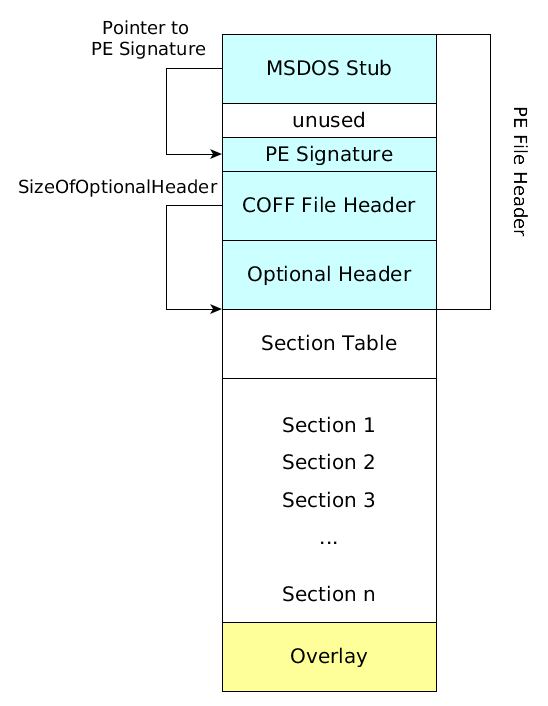
\includegraphics[width=.98\textwidth, height=.60\textheight,keepaspectratio]{graphics/peformat}
\caption{Structure of a PE file}
\label{fig:peformat} 
\end{figure}

\autoref{fig:peformat} illustrates the structure of a \PE{} file. It consists of the so called PE Header, followed by the Section Table and the sections. The overlay is optional data appended to the file. As different resources use the term \emph{PE Header} with variable meanings \todo{or not use it commonly}, the following defintion by the \PECOFF{} will be used in the following: \todo{avoid konjunktivb}

\begin{definition}[PE Header]
The \emph{PE Header} \enquote{consists of a MS-DOS stub, the PE signature, the COFF file header, and an optional header.} \cite[\p{11}]{pespec}
\end{definition} 

The different parts of the \PE{} are explained hereafter.

A \PE{} file always starts with the MS-DOS Stub. This is an application which is able to run in MS-DOS. The standard MS-DOS Stub prints the message \enquote{This program cannot be run in DOS mode} and closes right after. 

The operating system determines the file format by looking for specific signatures. The file format signature is usually at the very beginning of the file. Since the \PE{} starts with the MS-DOS Stub, which has a file format signature itself, the \PE{} signature is placed after. \todo{MZ, PE00} The offset to the \PE{} signature is defined in location 0x3c of the MS-DOS Stub, thus enables Windows to properly execute the \PE{} file. Right after the PE signature follows the PE Header.

The first part of the PE Header is the COFF File Header. It contains information about the type of the target machine, the number of sections, a time date stamp that indicates when the file was created, the size of the Optional Header and flags that indicate file characteristics including a flag that indicates whether the file is a \DLL{}\label{dllflag}.

The Optional Header follows right after the COFF File Header at a certain offset from the beginning of the PE Header. Despite its name the Optional Header is mandatory for image files. Only object files don't need it. The Optional Header has three parts: Standard Fields, Windows Specific Fields and a Data Directory Table.

The Standard Fields of the Optional Header contain information necessary for loading and running the file. They determine for example, whether the image file allows a 64-bit address space (\PEplus{}) or is limited to a 32-bit address space (\PEsmall{}). They also declare \ia{} the size of initialized and uninitialized data, the size of the code, the linker versions and the entry point (see \autoref{def:entrypoint}) of the image file.

The Windows Specific fields provide additional information for the Windows loader and linker like the operating systems the image file can run on, alignment values, dll characteristics and the number of data directories in the Data Directory Table.

A Data Directory Table entry consists of address and size for a table or string that the system uses. Examples are the import table, the export table and the resource table. (see \cite[\pp{24}]{pespec})

The Section Table is placed right after the Optional Header. It consists of the section headers for the sections that make up the rest of the \PE{} file. A section header describes \ia{} characteristics, size, name and location of a section.

While the PE Header and Section Table described above are located at a fixed file offset, the rest of the \PE{} contains data defined by pointers in the PE Header or the Section Table. The sections contain arbitrary data, only some sections have a special meaning and are explained in \emph{\nameref{sec:specialsections}} below. An \EXE{} file has at least one section containing executable code.

Data that was appended to the file, but is not part of the \PE{} format is called \emph{overlay}. Overlay is not mapped into memory. The overlay is used by some applications as a way to store arbitrary data without having to deal with the \PE{} format. 

\section{Special Sections} \label{sec:specialsections}

Sections may contain arbitrary information, which is only relevant to the application using them; but some sections have a special meaning. Their format is described in the \PECOFF{} \cite{pespec}. These sections are recognized by entries in the Data Directory Table of the Optional Header or certain flags in the Section Table. They have typical section names which are also used in the \PECOFF{} to refer to the sections. These names are not mandatory, but a convention. That's why they can not be relied on while trying to find certain sections in a \PE{}. Not only malware writers misuse the section names to obscure their purpose, but also legimate compilers and packers violate the convention. \todo{example!}
Some of these special sections are described right after. \todo{sections that are recognized by portex}

\subsection*{Export Section} \label{subsec:idata}

The \emph{.edata Section} or \emph{Export Section} is generally found in \useacronym[s]{DLL}. The section begins with the Export Directory Table, which contains general information and addresses to resolve imports from this section. The Export Directory Table points to an array of addresses called Export Address Table. Each address either points to code or data within the current image file, or is a forwarder address which points to a symbol in another \DLL{}. 

Other image files have two ways to import symbols from the current image file: They either use an index into the Export Address Table (the index is also called \emph{ordinal}) or they use a public name of the symbol. Ordinals are defined in the Ordinal Table; public names are defined in the Export Name Table.

Entries of the Ordinal Table correspond to the Export Name Pointer Table entries by their position. Every entry is an ordinal that represents an index in the Export Address Table.

The Export Name Pointer Table is an array of addresses which point to names of the Export Name Table. These names are null-terminated ASCII strings. They are the public names that other image files can use to import the symbols.

\autoref{lst:exportsample} shows example contents for a \DLL{} with two exported symbols: \texttt{DLL2Print} and \texttt{DLL2ReturnJ}. It also illustrates in lines 34-40 how the information from the different tables is combined.

\lstinputlisting[caption={Example for Export Section contents, output by \portex{}},captionpos=t,label=lst:exportsample]{listings/edata_sample}

\subsection*{Import Section}

\begin{figure}
\centering
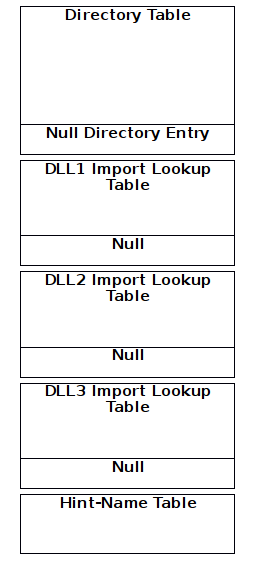
\includegraphics[width=.98\textwidth, height=.60\textheight,keepaspectratio]{graphics/importsection}
\caption{Typical Import Section Layout by \protect{\cite[\p{61}]{pespec}}}
\label{fig:import} 
\end{figure}

Every image file that imports symbols has an \emph{Import Section}, also called \emph{.idata Section}.
The Import Section contains the Import Directory Table, several Import Lookup Tables, the Hint-Name Table and the \IAT{}. A typical layout of the Import Section is in \autoref{fig:import}

Every Import Directory Table entry points to an Import Lookup Table. Each Import Lookup Table describes the imported symbols of a single \DLL{}.

The Hint-Name table entries have a hint and an ASCII name of the import. Each hint is an index to the Export Name Pointer Table (see \autoref{subsec:idata}) of the \DLL{} the image is importing from. Hints speed up the lookup of imports.

Null entries mark the end of the Import Directory Table and the Import Lookup Table.

The \IAT{} is identical to the Import Directory Table except while the image is bound. In the latter case the \IAT{} entries are overwritten with memory addresses of the imported symbols.

\subsection*{Resource Section}

Resources of a \PE{} can be \ia{} icons, text, windows, copyright information. They are saved as an entry in the \emph{Resource Section}, which also has the name \emph{.rsrc Section}. The Resource Section is build up as a tree with the actual resource addresses as leaves. While \(2^{31}\) tree levels can be used according to the \PECOFF{} \cite[\p{100}]{pespec}, Windows only uses three levels with the first level node being the type, the second being the name and the third being the language information. \autoref{fig:resourcetree} illustrates the structure of a resource tree.

\begin{figure}
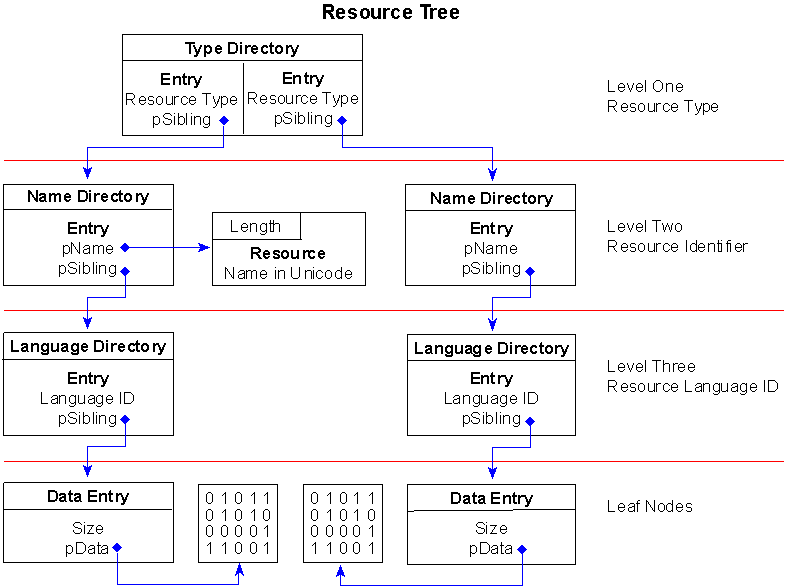
\includegraphics[width=.98\textwidth, height=\textheight,keepaspectratio]{graphics/resourcetree}
\caption{ Resource tree structure by \protect{\cite{kath13}}}
\label{fig:resourcetree} 
\end{figure}

\subsection*{Debug Section and Debug Directory}

Whereas most sections can be at an arbitrary location in the file, the \emph{Debug Section} (aka \emph{.debug Section}) must be placed at the very end of the image file. The reason is that the loader doesn't map this section into memory. Image files contain per default of the linker only a Debug Directory (as pointed to by the Data Directory Table), but not a Debug Section (see \cite[\p{78}]{pespec}). Thus the Debug Directory is either located in the Debug Section if it exists, in any other section of the \PE{} or not in any section at all.

Every Debug Directory entry defines \ia{} size, location and the type (format) of a debug information block. An example is in \autoref{lst:debugsample}

\lstinputlisting[caption={Example for a Debug Section entry, output by \portex{}},captionpos=t,label=lst:debugsample]{listings/debug_sample}

\section{Loading Process}

test \cite{peloading} why?

\begin{sidewaysfigure}
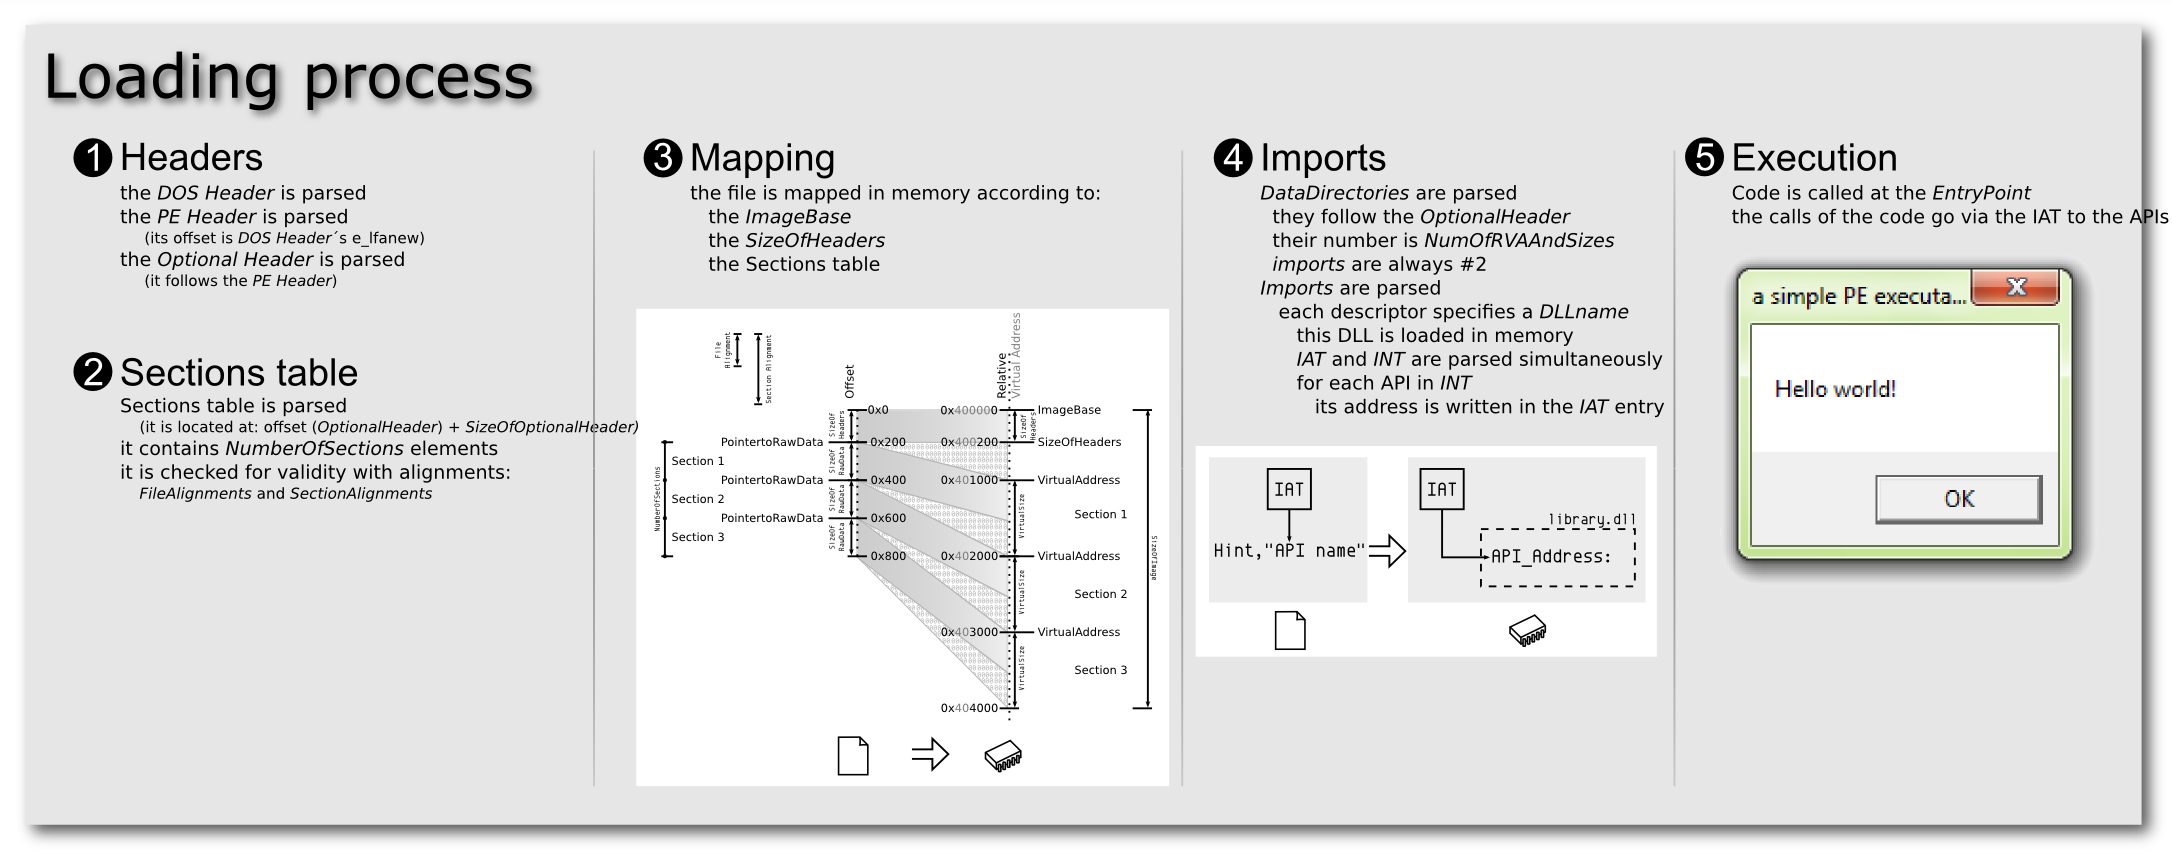
\includegraphics[height=.39\textheight,keepaspectratio]{graphics/pe101}
\caption{ Loading Process of a PE by \protect{\cite{peloading}}. Note that the term PE Header is used synonymously to COFF File Header in this graphic}
\label{fig:loading} 
\end{sidewaysfigure}

\todo{add reference to figure}

\section{PE Malformations}

\begin{definition}[Malformation]
A \emph{malformation} is data or layout of a \PE{} file that violates the \PECOFF{}.
\end{definition} 

Malformations are either accidental results of \PE{} modifications or done on purpose.
A malformation doesn't necessarily prevent the Windows loader from running the file. The Windows loader doesn't work in full compliance with the \PECOFF{} to maintain backward compatibility with obsolete compilers and files. Malware writers utilize the loader's behaviour to create normally working \PE{} files that can not be parsed by most tools used for malware analysis. Some malformations, like setting reserved fields, are also done to hide information in a \PE{}; for example marking a host file as infected to prevent a virus from infecting it twice.

Accidental malformations occur if the malware writer doesn't know the \PECOFF{} enough to perform modifications in compliance with it. An example is a virus that spreads by adding a new section to the host file, copying the own code into it and changing the entry point to the beginning of the new section. The changes done to the host file can lead to subsequent malformations without impairing the Windows loader while running the file.

Sheehan et\thinspace{}al states that 68~\% of all image files have malformations. \cite[slide 7]{sheehan07}
Because \portex{} specializes in \PE{} malware, one goal of \portex{} is to parse malformated \useacronym[s]{PE} correctly and to recognize malformations.

%While other sources only use the term malformation for a file that still runs normally, this is not a premise for this thesis. If modifications to a \PE{} done by malware lead to a non-working host file, the file might still be of interest for malware analysis. \portex{} shall still be able to get as much information of the file as possible despite the damage done to the file. \todo{ausdruck? remove paragraph?}

The following malformation examples are modifications done on purpose to deceive malware analysis tools.

\subsection{Simple Malformations}

A malformation is \emph{simple} if it concerns a single field or data table in the \PE{} (\cf{} \cite[slide 7]{vuksan11}).
The malformation examples described hereafter are in ascending order of their complexity. \todo{remove?}

\subsubsection*{No Sections}

\subsubsection*{Too Many Sections}

\subsubsection*{PE Header in Overlay}

The PE Header usually follows after the MS-DOS Stub \todo{pespecreferences, usual vs change}

As explained in \autoref{sec:pestructure} the address to the beginning of the PE signature and the following PE Header is located in file offset 0x3c within the MS-DOS Stub. This address is a 32-bit value and can be changed to point to the overlay of the file as illustrated in \autoref{fig:overlayheader}. (\cf{} \cite[slide 13]{vuksan11})

\begin{figure}
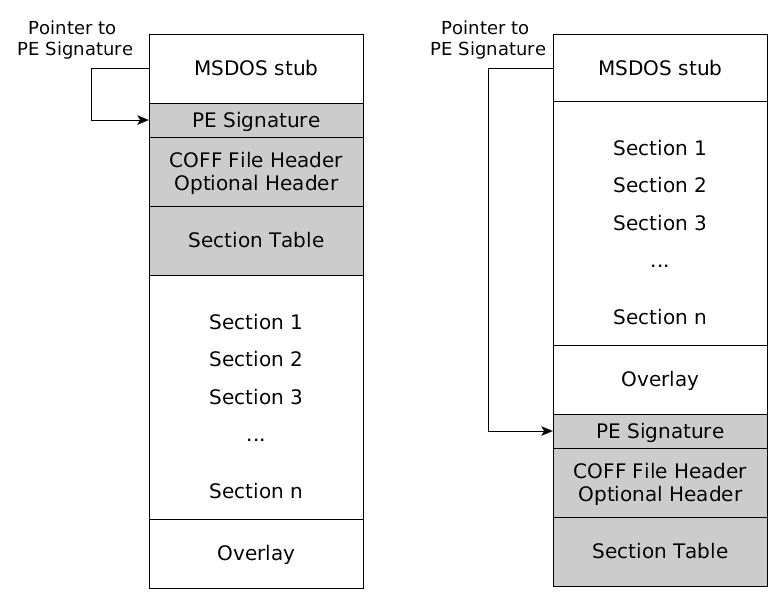
\includegraphics[width=.98\textwidth, height=.60\textheight,keepaspectratio]{graphics/overlayheader}
\caption{PE Header in Overlay \protect{(\cf{} \cite[slide 13]{vuksan11})}}
\label{fig:overlayheader} 
\end{figure}

Reverse Engineering tools that expect the PE Header to be in its standard location at a certain range from the beginning of the file will have difficulties to parse a \PE{} with this malformation.

\subsubsection*{Section Table in Overlay}

The idea from the previous malformation is extended by moving only the Section Table to the overlay. The Optional Header has a variable size. The offset from the beginning of the Optional Header and its size determine the beginning of the Section Table. The size is defined in the field \texttt{SizeOfOptionalHeaders} the COFF File Header. It is a 16-bit value, so the maximum value for the size is 65535. If the end of the file is smaller than the offset of the Optional Header plus its size, the Section Table can be moved to the very end of the file. \autoref{fig:overlaysectable} illustrates the malformation.

As a result of this modification the Section Table will not be mapped to memory. A tool that parses the memory content will not be able to find the Section Table. Pericin demonstrates this in his talk at the BlackHat Conference with the debugger OllyDbg. \cite[min.\thinspace{}14:45]{vuksan11} 

\begin{figure}
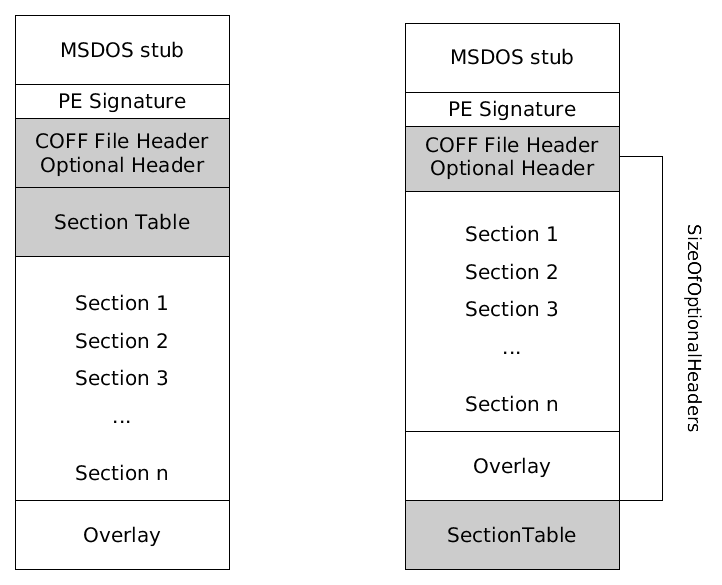
\includegraphics[width=.98\textwidth, height=.60\textheight,keepaspectratio]{graphics/overlaysectable}
\caption{Section Table in Overlay \protect{(\cf{} \cite[slide 14]{vuksan11})}}
\label{fig:overlaysectable} 
\end{figure}

\subsubsection*{Dual Data Directories}

The \texttt{SizeOfHeaders} field in the Optional Header defines the \enquote{combined size of an MS-DOS Stub, PE header, and section headers} \cite[\p{20}]{pespec}. But it also determines the \VA{} of the first section implicitly. \cite[slide 15]{vuksan11} 

If the \texttt{SizeOfHeaders} field is modified to a smaller value, the modification will result in loading only part of the PE Header to memory. Most of the PE Header will still be processed on disk regardless of the \texttt{SizeOfHeaders} field, including the Section Table. So setting the \VA{} of the first section in the Section Table to the same value of the \texttt{SizeOfHeaders} field will make the section part of the PE Header in memory. 
The Data Directory Table is parsed from memory by the operating system. That means writing a different continuation of the PE Header to the first section will result into \eg{} different imports or exports used by the operating system than the ones parsed on disk by reverse engineering tools.

\todo{figure}

\subsection{Complex Malformations}

A malformation is complex if it concerns multiple fields or data tables in the \PE{} (\cf{} \cite[slide 7]{vuksan11}).
